\documentclass[11pt,paper=a4,final]{scrartcl}
\usepackage[utf8]{inputenc}
\usepackage{geometry}           %allows us to specify the 'seitenrand'
\usepackage{graphicx}           %package used to include graphics
\usepackage{hyperref}           %used to make klickable links
\usepackage{listings}
\usepackage{tabularx}
\usepackage{pdflscape}
\usepackage[figuresright]{rotating}
\usepackage{nameref}
\usepackage{longtable}
\usepackage{enumitem}
\usepackage{ngerman} % Make the document German
\usepackage[table]{xcolor}
% Make the document German
\usepackage{ngerman}
\usepackage{fancyhdr}
\usepackage{lipsum}
\usepackage{mdwlist}
\usepackage{multirow}
\usepackage{moreverb}

\hypersetup{
    colorlinks,
    citecolor=black,
    filecolor=black,
    linkcolor=black,
    urlcolor=black
}


\title{Arbeitsjournal}
\author{Niklaus Hofer, Roland Rytz}
\date{\today{}}

% Make title and author accessible in the header/footer
\makeatletter
  \let\Title\@title
  \let\Author\@author
\makeatother

\pagestyle{fancy}

\geometry{a4paper, top=20mm, right=20mm, bottom=30mm, left=20mm}

\fancyhf{}      %delete default values
\setlength{\headwidth}{\textwidth}      %header and footer width equal the text width
\lhead{\Author}
\rhead{\Title}
\fancyfoot[CE,CO]{Speicherdatum: \today{}}
\fancyfoot[RE,RO]{\thepage}

\begin{document}
\maketitle
\newpage
\begin{abstract}
\end{abstract}
\section{Dokumenteninformationen}
\subsection{\"Anderungskontrolle}
\subsection{Referenzierte Dokumente}
\subsection{Verwendete Abk\"urzungen}
\tableofcontents
%\listoffigures
%\listoftables
\section{Managementsummary}
\subsection{Aufgabenstellung}
Unser Programm soll den Vigenere-Algorithmus visuell erkl\"aren. Ein
Wikipedia-Artikel soll die n\"otigen Hintergrundinformationen zu dem Thema
bereit halten. In Englischer Sprache gibt es bereits seit L\"angerem einen
Artikel zu dem Tema, nicht so in der deutschen Wikipedia.
\subsection{Varianten}
Gerade in der Webentwicklung gibt es sehr viele unterschiedliche Tools und
Ans\"atze. Es ist wichtig, dass man sich von Beginn weg f\"ur den am besten
geeigneten Prozess und gute Werkzeuge entscheidet. In diesem Abschnitt werden
die M\"oglichkeiten aufgezeigt und der Entscheid begr\"undet.
\subsection{Konzept}
Hier finden die Planung der Produkte statt. Der Aufbau der Applikation wird
geplant und aufgezeigt. Die Struktur des Wikipedia-Artikels wird geplant. Hier
werden sich auch erste Ablauf-Diagramme und Vorlagen finden.
\subsection{Realisierung}
Im Verlauf der Arbeiten an den Produkten treten Unterschiede zu der Planung auf
die sich zumeist aus unvorhergesehenen Komplikationen oder Vereinfachungen
ergeben. Alle Unterschiede zur Planung werden hier erl\"autert und begr\"undet.
\subsection{Mittelbedarf}
Hier werden die n\"otigen Ressourcen aufgelistet.
\subsection{Fazit}
%TODO
\part{Ablauf und Umfeld}
\section{Projektmethode Hermes}
\begin{figure}[htb!]
  \centering
  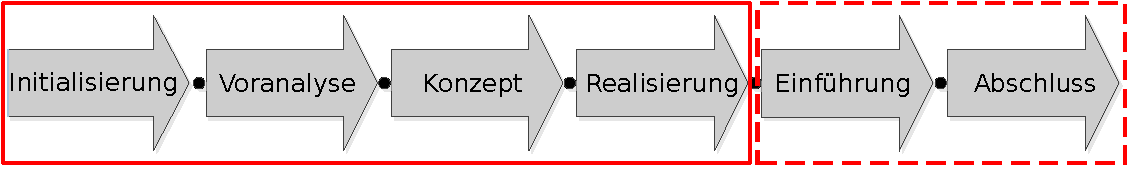
\includegraphics[width=\textwidth]{hermes.pdf}
  \caption{Hermes Light Schema}
  \label{fig:hermes_schema}
\end{figure}
Wir haben die Projektmethode Hermes Light gew\"ahlt. Hermes Light ist eine
vereinfachte und verkürzte Variante von Hermes. In der Grafik
\ref{fig:hermes_schema} sind die sechs Phasen der Projektmethode aufgezeigt. Die
letzten zwei Phasen, \glqq Einführung\grqq und \glqq Abschluss\grqq werden im
Rahmen dieser IPA nur teilweise durchgeführt. Die Einf\"uhrung besteht im
Bereitstellen der Webseite und des Artikels. Der Abschluss allerdings wird hier
nur beschrieben.

In den Abschnitten unten, werden wird die jeweilige Phase kurz erläutern und
aufzeigen welche Teile dieses Dokumentes zu welcher Phase gehören.
%\newpage
\subsection{Initialisierung}
\begin{itemize*}
  \item Festlegung eines klar definierten organisatorischen und technischen
  Rahmens als Voraussetzung für eine erfolgreiche Projektabwicklung
  \item Planung, Vernehmlassung und Beurteilung des Projekts
  \item Freigabe der Phase Voranalyse
\end{itemize*}
Diese Phase beinhaltet folgende Punkte dieser Dokumentation:
% TODO
\begin{itemize*}
  \item 
\end{itemize*}
\subsection{Voranalyse}
\begin{itemize*}
  \item Erstellung und Beurteilung der Situationsanalyse sowie Überprüfung der
  Zielsetzungen, der Problemstellung und des Untersuchungsbereichs
  \item Erarbeitung von Lösungsvorschlägen und Abschätzung ihrer
  voraussichtlichen Wirtschaftlichkeit und Realisierbarkeit
  \item Auswahl eines Lösungsvorschlages und Freigabe der Phase Konzept.
\end{itemize*}
Diese Phase beinhaltet folgende Punkte dieser Dokumentation:
% TODO
\begin{itemize*}
  \item 
\end{itemize*}
% TODO
Eigentlich beinhaltet diese Phase noch die Punkte \glqq Termine\grqq und \glqq
Zeitplan\grqq . Aufgrund des Ablaufs der IPA und da diese Daten gegeben sind,
habe ich oben genannte Punkte aber in die Phase Initialisierung verschoben.
\subsection{Konzept}
\begin{itemize*}
  \item Vollständige Darstellung des Systems, ausgehend vom gewählten Lösungsvorschlag
  \item Beurteilung kritischer Teilsysteme
  \item Freigabe der Phase \glqq Realisierung\grqq
\end{itemize*}
Diese Phase beinhaltet folgende Punkte dieser Dokumentation:
% TODO
\begin{itemize*}
  \item 
\end{itemize*}
Die Konzeptphase widmet sich der konkreten Gestaltung des Systems. Es beinhaltet
die Struktur, die Architektur, das Design, sowie die Funktionalitäten der zu
entwickelnden Applikation.
\subsection{Realisierung}
\begin{itemize*}
  \item Erkläuterungen zum geschriebenen Code
  \item Aufzeigen und Begründen von Änderungen gegenüber dem Konzept
  \item Freigabe der Phase Einführung
\end{itemize*}
Diese Phase beinhaltet folgende Punkte dieser Dokumentation:
% TODO
\begin{itemize*}
  \item 
\end{itemize*}
\subsection{Einf\"uhrung}
%TODO
\subsection{Abschluss}
%TODO
\section{Aufgabenstellung}
\subsection{Ausgangslage}
Der Vigenere-Algorithmus ist bereits mehrere Hundert Jahre alt. Er ist
einerseits intuitiv und auch f\"ur Laien leicht verst\"andlich. Trotzdem lassen
sich daran einige wichtige Punkte von kryptografischen Systemen aufzeigen. Trotz
der schnell verst\"andlichen St\"arken des Algorithmus l\"asst er sich heute mit
sehr wenig Aufwand knacken. 

Die meisten Webseiten die Vigenere grafisch erkl\"aren tun die mit Hilfe eines
Java-Applets. Im Zeitalter von HTML5 ist der Einsatz von Java-Applets auf
Webseiten aber fragw\"urdig und stark umstritten. Wir m\"ochten diese veralteten
Versionen der grafischen Darstellung des klassischen Algorithmus durch eine
zeitgerechte Web-Applikation in HTML/CSS/JS ersetzen.

Auf der Englisch-sprachigen Wikipedia findet sich ein separater Artikel zu
Vigenere's Algorithmus. In der Deutschen Wikipedia hingegen ist lediglich ein
Artikel zu finden, der das Gebiet in einem breiteren Spektrum abdeckt und zu
Vigenere nur wenige Informationen bietet. Dies m\"ochten wir mit einem Eintrag
speziell zu diesem Tema \"andern.
\subsection{Auftragsformulierung}
\begin{table}[h!]
  \centering
  \begin{tabular}{|p{4cm}|p{12cm}|}\hline
    \bf Oberthema & (NULL) \\ \hline
    \bf Arbeitstitle & Visualiesierung Vigenère Chiffre und
    Krypto-AnalyseVisualiesierung Vigen\'ere Chiffre und Krypto-Analyse \\
    \hline
    \bf Zielsetzungen & Implementation und Visualisierung der Funktionsweise
    eines Vigenère Algorithmus. Verfassen eines dedizierten Wikipedia-Artikels
    zu dem Thema auf Deutsch. \\ \hline
    \bf Leitfragen & \begin{itemize*} \item Wie koennen einfache, kryptografische
    Ablaeufe visualisiert und erklaert werden? \item Wie funktioniert der
    Vigen\'ere Algorithmus? \item Wieso gilt der einst als unknackbar
    bezeichnete Algorithmus heute als unsicher? \end{itemize*} \\ \hline
    m\"ogliches \bf Produkt & \begin{itemize*} \item Visualisierung des Vigen\'ere
    Algorithmus mit Javascript/HTML/CSS \item Deutscher Wikipedia Artikel zu dem
    Thema des Vigen\'ere Algorithmus \end{itemize*} \\ \hline
    \bf Adressaten & \begin{itemize*} \item Technik- und Kryptografie
    Interessierte \item Leser der Wikipedia \end{itemize*} \\ \hline
    Stichwörter zum geplanten Vorgehen & Vigen\'ere, Wikipedia, Kryptografie,
    Verschluesselung, Wissensvermittlung, Visualisierung \\ \hline
    \bf Beteiligte Schulf\"acher & \begin{itemize*} \item Mathematik \item
    Deutsch \end{itemize*} \\ \hline
    \bf Zweitkorrigierende Lehrkraft & Herr G. L\"uthi \\ \hline
  \end{tabular}
  \caption{Auftragsformulierung}
  \label{tab:auftrag}
\end{table}
\newpage
\subsection{Mittel und Methoden}
\begin{table}[h!]
 \centering
  \begin{tabular}{|p{4cm}|p{12cm}|}
  \hline
  Projektmethode & Hermes Light, Eine auf den Projektumfang zugeschnittene
  Variante von Hermes \\ \hline Systeme & Computer zum Schreiben des Codes.
  Internetanschluss \\ \hline Testing environment & System das in der Lage ist,
  virtuelle Mascheinen auszuf\"uhren zum Testen mit verschiedenen Browsern unter
  verschiedenen Systemen \\ \hline Entwicklungssoftware & Editor, Browser,
  Javascript, JQuery \\ \hline Dokumentation & Texteditor, pdflatex, MikTex \\
  \hline Entwicklungssprache & Javascript \\ \hline Versionsverwaltung & git,
  github \\ \hline
  \end{tabular}
  \caption{Auflistung der Mittel und Methoden}
\end{table}
\subsection{Projektorganisation}
\begin{figure}[h!]
  \centering
  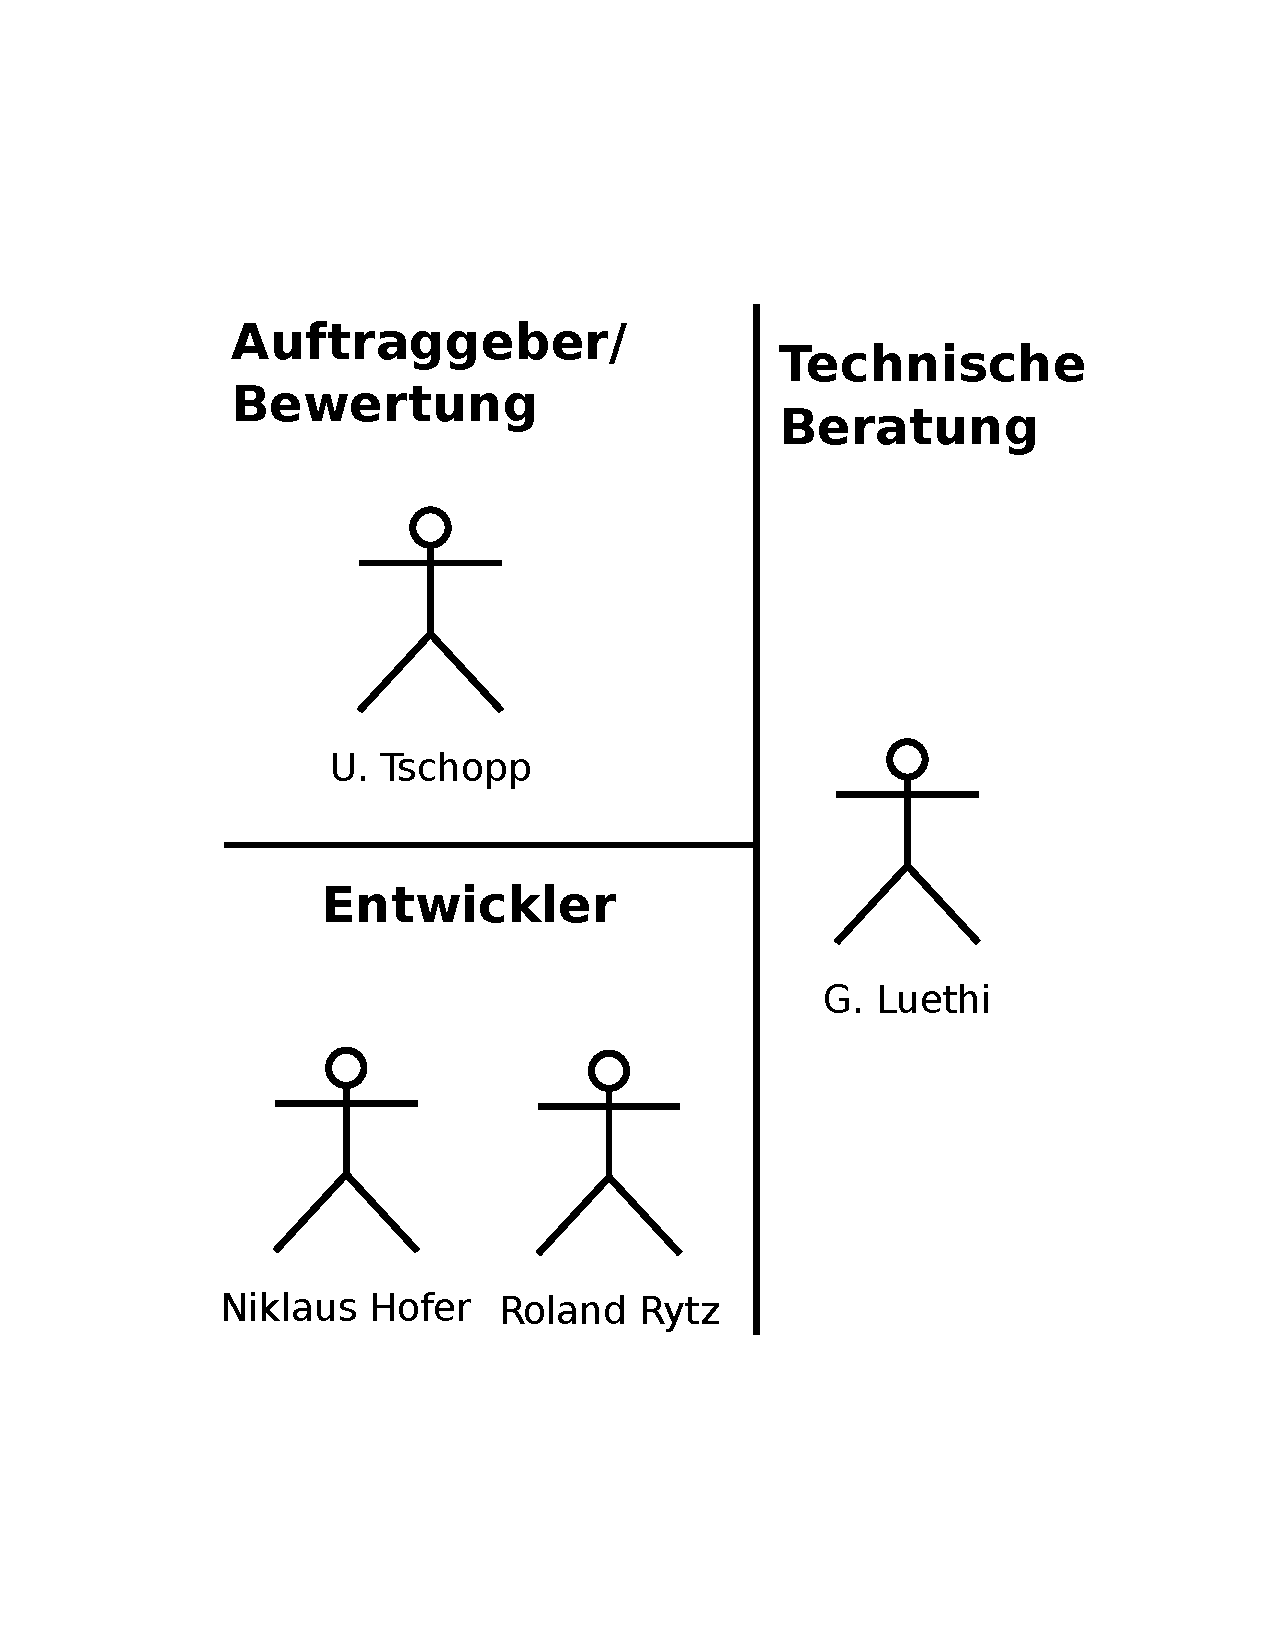
\includegraphics[width=0.6\textwidth]{rollen.pdf}
  \caption{Projektrollen, Visualisierung}
  \label{fig:projektrollen}
\end{figure}
\newpage
\subsection{Projektrollen}
\begin{table}[h!]
  \centering
  \begin{tabular}{|l|l|l|}
    \hline
    \bf Funktion & \bf Person & \bf Beschreibung \\ \hline
    Auftraggeber & Herr Tschopp & Lehrkraft \\ \hline
    Projektleiter & Niklaus Hofer & \\ \hline
    Fachberater Mathematik & Herr L\"uthi & Lehrkfraft \\ \hline
    Fachberater Deutsch & Herr Tschopp & Lehrkraft \\ \hline
    Entwickler & Roland Rytz & \\ \hline
    Entwickler & Niklaus Hofer & \\ \hline
  \end{tabular}
  \caption{Projektrollen}
\end{table}
\section{Vorkenntnisse}
Roland Rytz ist erfahrener Javascript Entwickler. Im Verlauf seiner Berufslehre
als Informatiker EFZ hat er zahlreiche Webseiten und Webapplikatione mit
Javascript realisiert. Roland hat dann auch in diesem Bereich seine
Abschlussarbeit geschrieben Auch in der Freizeit hat Roland bereits einige
Webseiten geschrieben. JQuery, die Webentwicklungswerkzeuge von Googles Chrome
Browser und Firefox FireBug sind vertraute Werkzeuge. Auch das Testen mit
verschiedenen Browsern ist keine Neuheit.

Niklaus Hofer hat bereits einfache Vigenere Implementationen in C++, Python und
Java geschrieben und sich kurz theoretisch mit dem Thema auseinandergesetzt.

Die beiden Autoren sind theoretisch mit dem Erstellen von Wikipedia-Artikeln
vertraut, haben aber noch nie zuvor eigene Artikel verfasst.
\section{Vorarbeiten}
Es gibt zu dieser Arbeit keine Vorarbeiten.
\section{Termine}
\begin{table}[h!]
  \centering
  \begin{tabular}{|l|l|}\hline
    Projektstart & Somewhen in August/September 2012 \\ \hline
    Abgabepermin & Freitag, 25. Januar 2012 \\ \hline
    Kontrolle Arbeitsjournal & 29. November 2012 \\ \hline
    Kontrolle Arbeitsjouranl & 21. Dezember 2012 \\ \hline
    1. Termin mit Herr L\"uthi & 13. November 2012 \\ \hline
    2. Termin mit Herr L\"uthi & 8. Januar 2013 \\ \hline
  \end{tabular}
  \caption{Termine}
  \label{tab:termine}
\end{table}
\begin{landscape}
  \section{Arbeitsjournal}
  Datum im Format Jahr.Monat.Tag
  \begin{longtable}{|p{1.8cm}|p{1.5cm}|p{5.0cm}|p{11.0cm}|l|l|}
    \hline
    \multirow{2}{*}{\bf Datum} & \multirow{2}{*}{\bf Wer} &\multirow{2}{*}{\bf T\"atigkeit} & \multirow{2}{*}{\bf Reflexion} & \multicolumn{2}{c|}{\bf Zeit} \\ \cline{5-6}
     & & & & \bf Geplant & \bf Effektiv \\ \hline
    %Use the headings below if you don't have multirow installed
    %\bf Datum & \bf Wer & \bf T\"atigkeit & \bf Reflexion & \bf Geplant & \bf Effektiv \\ \hline
    \hline
    \endhead
    % Beginn section ---------------------------------------------------------
    2012.09.09 & Niklaus und Roland &
    Initialisierung des Repositories. &
    Die Zusammenarbeit funktioniert bis jetzt gut. &
    20min & 20min \\ \hline \nopagebreak
    \multicolumn{2}{|l|}{\bf Pendenzen} &\multicolumn{2}{p{16.0cm}|}{Planen des weiteren Vorgehens.}  & \multicolumn{2}{l|}{} \\ \hline
    % End section ------------------------------------------------------------
    % Beginn section ---------------------------------------------------------
    \hline
    2012.10.19 & Niklaus und Roland &
    Schreiben des ersten Programmcodes. Erstellen des Vigenere square mit HTML und Javascript. &
    Der Wiedereinstieg in die Progammierung ist nicht ganz einfahc gefallen. Wir hatten deshalb deutlich l\"anger als urspr\"unglich geplant und sind auch nicht so weit fortgeschritten wie geplant. &
    30min & 80min \\ \hline \nopagebreak
    \multicolumn{2}{|l|}{\bf Pendenzen} &\multicolumn{2}{p{16.0cm}|}{Wir wollen die grundlegenden Funktionen implementieren, damit wir beim ersten Gespr\"ach mit Herr L\"uthi bereits etwas zeigen k\"onnen. Insbesondere die 'sichtbaren' Funktionen sollten dann da sein. Das GUI muss dann aber nat\"urlich noch nicht fertig sein.}  & \multicolumn{2}{l|}{} \\ \hline
    % End section ------------------------------------------------------------
    % Beginn section ---------------------------------------------------------
    \hline
    2012.10.19 & Niklaus &
    Implementieren des Verschl\"usselungsalgorithmus in Javascript. Testen der Verschl\"usselung, Vergleich mit einer anderen (online verf\"ugbaren) Vigenere Implementationen.&
    Am Nachmittag konnte ich nach Langem wieder einmal programmieren. Das hat mich nicht mehr losgelassen. Ich habe also die Verschl\"usselung implementiert. Das ist mir \"uberraschend schnell gelungen, insbesondere wenn man bedenkt, dass ich zuvor kaum jemals mit Javascript gearbeitet habe. Die Verschl\"usselung implementiert lediglich den Algorithmus und stellt nichts grafisch dar. Sie kann aber genutzt werden um den mathematischen Aspekt des Projektes hervorzuheben. Ein Geschwindigkeitsvergleich zwischen der Methode mit dem manuellen Auslesen der Charaktere aus dem Square und der mathematischen Funktion, sollte die Vorz\"uge der wesentlich schnelleren, mathematischen Funktion deutlich hervorheben.&
    60min & 120min \\ \hline \nopagebreak
    \multicolumn{2}{|l|}{\bf Pendenzen} &\multicolumn{2}{p{16.0cm}|}{}  & \multicolumn{2}{l|}{} \\ \hline
    % End section ------------------------------------------------------------
    % Beginn section ---------------------------------------------------------
    2012.10.22 & Niklaus &
    Implementation des Verschl\"usselungsalgorithmus.&
    In der Pause im Mathematikunterricht habe ich die Entschl\"usselung implementiert. Das war eine schlechte Idee, ich konnte mich danach nicht mehr auf den Unterricht konzentrieren. Im weiteren Verlauf des Nachmittags ist mir eingefallen, wie ich den Code besonders sch\"on machen kann. Da die Entschl\"usselung \"ahnlich der Verschl\"usselung ist, konnte ich viel Code \"ubernehmen und ben\"otigte weniger Zeit.&
    15min & 30min \\ \hline \nopagebreak
    \multicolumn{2}{|l|}{\bf Pendenzen} &\multicolumn{2}{p{16.0cm}|}{}  & \multicolumn{2}{l|}{} \\ \hline
    % End section ------------------------------------------------------------
    % Beginn section ---------------------------------------------------------
    \hline
    2012.10.22 & Roland &
    Portieren des vorhandenen Codes nach JQuery. Der Code zur Generierung des Squares wird in ein Objekt \"ubernommen, dem sp\"ater verschiedene Funktionen hinzugef\"ugt werden k\"onnen.&
    Die Javascript Programmierung wird durch die Verwendung von JQuery erleichtert. Die objektorientierte Programmierung ist zeitgem\"ass und bringe ebenfalls viele Vorteile mit sich.&
    30min & 30min \\ \hline \nopagebreak
    \multicolumn{2}{|l|}{\bf Pendenzen} &\multicolumn{2}{p{16.0cm}|}{Funktionen zum Highlighten der richtigen Spalten und Zeilen m\"ussen noch geschriben werden, damit die Verschl\"usselung grafisch dargestellt werden kann. Ausserdem m\"ussen die entsprechenden Werte ausgelesen werden. Danach sollten wir bereit f\"ur eine erste Besprechung mit Herr L\"uthi sein.}  & \multicolumn{2}{l|}{} \\ \hline
    % End section ------------------------------------------------------------
    % Beginn section ---------------------------------------------------------
    \hline
    2012.10.22 & Roland &
    Implementieren des Highlightings im Square.&
    Im Square k\"onnen einzelne Spalten und Linien gezielt markiert wreden. Ausserdem k\"onnen Buchstaben aus dem Schnittpunkt ausgelesen werden.&
    30min & 30min \\ \hline \nopagebreak
    \multicolumn{2}{|l|}{\bf Pendenzen} &\multicolumn{2}{p{16.0cm}|}{}  & \multicolumn{2}{l|}{} \\ \hline
    % End section ------------------------------------------------------------
    % Beginn section ---------------------------------------------------------
    \hline
    2012.10.31 & Roland &
    Versch\"onern der Highlight Funktion.&
    &
    40min & 40min \\ \hline \nopagebreak
    \multicolumn{2}{|l|}{\bf Pendenzen} &\multicolumn{2}{p{16.0cm}|}{}  & \multicolumn{2}{l|}{} \\ \hline
    % End section ------------------------------------------------------------
    % Beginn section ---------------------------------------------------------
    \hline
    2012.11.23 & Niklaus &
    Portieren des vorhandenen Protokolls (der Notizen) in eine richtige HERMES
    Struktur&
    Dies wird die Dokumentation deutlich \"ubersichtlicher machen.&
    45min & 45min \\ \hline \nopagebreak
    \multicolumn{2}{|l|}{\bf Pendenzen} &\multicolumn{2}{p{16.0cm}|}{HERMES ist
    ein komplexer Standard. Das wird noch einiges an Zeit in Anspruch nehmen.}  & \multicolumn{2}{l|}{} \\ \hline
    % End section ------------------------------------------------------------
    % Beginn section ---------------------------------------------------------
    \hline
    2012.11.23 & Niklaus Hofer &
    Besprechung mit Herr Tschopp \"uber den Projektstand und das geplante
    weitere Vorgehen. & Bis jetzt siehts nicht schlecht aus. Wir sind gut im
    Zeitplan. Allerdings sollten wir mit dem Erstellen des Wikipedia-Artikels
    beginnen. Wir haben abgemacht, dass ein Entwurf der Struktur des Artikels
    anfangs Dezember vorliegen sollte. Um diese Struktur zu erstellen, werden
    wir andere Wikipedia-Artikel zu \"ahnlichen Themen auf ihren Aufbau
    untersuche. Die Resultate werden wir festhalten und uns dann beim Erstellen
    des eigenen Artikels daran orientieren.&
    40min & 20min \\ \hline \nopagebreak
    \multicolumn{2}{|l|}{\bf Pendenzen} &\multicolumn{2}{p{16.0cm}|}{
      \begin{itemize*}
        \item Beginn der Arbeiten am Wikipedia-Artikel
	\begin{itemize*}
	  \item Erstellen des Rasters zum Untersuchen der Wikipedia-Artikel
	  \item Wikipediaartikel zu \"ahnlichen Themen untersuchen
	  \item Vorlage f\"ur den eigenen Artikel erstellen
	 \end{itemize*}
	 \item neuen Termin mit Herr L\"uthi vereinbaren
      \end{itemize*}
    }  & \multicolumn{2}{l|}{} \\ \hline
    % End section ------------------------------------------------------------
    % Beginn section ---------------------------------------------------------
    \hline
    2012.11.30 & Niklaus und Roland &
    Analyse von Wikipedia-Artikeln zu \"ahnlichen Themen. Erstellen einer
    Struktur f\"ur unseren eigenen Artikel in Abh\"angigkeit unserer
    Erkentnisse. Anlegen einer bibtex-Datenbank f\"ur die Referenzen.&
    Das Analysieren der Artikel nimmt deutlich mehr Zeit in Anspruch als
    geplant. Ausserdem m\"ussen wir aufpassen, dass wir uns an Artikeln
    \"ahnlichen Schwirigkeitsgrads orientieren. Solche zu Themen wie RSA oder
    AES (rejindael) sind vom Thema und folglich auch vom Aufbau her deutlich
    komplexer als solche zu einfacheren Algorithmen.
    &
    45min & 90min \\ \hline \nopagebreak
    \multicolumn{2}{|l|}{\bf Pendenzen} &\multicolumn{2}{p{16.0cm}|}{Als
    n\"achstes wollen wir die Analyse der Artikel fertigstellen, damit wir in
    den Ferien an dem Artikel arbeiten k\"onnen.
    }  & \multicolumn{2}{l|}{} \\ \hline
    % End section ------------------------------------------------------------
    % Beginn section ---------------------------------------------------------
    \hline
    2012.12.13 & Roland &
    Visuelles Ausgestalten des Webtools. Grafischer Modus wurde mit dem
    mathematischen Modus zusammengef\"uhrt, es kann nun ausgew\"ahlt werden,
    welcher Modus verwendet werden soll.&
    Zu viel Zeit wurde mit kleinen Details beim Ausgestalten der Grafischen
    Finessen aufgewendet.
    &
    15min & 60min \\ \hline \nopagebreak
    \multicolumn{2}{|l|}{\bf Pendenzen} &\multicolumn{2}{p{16.0cm}|}{
    Der grafische Modus hat noch einige kleinere Fehler, die noch behoben
    werden sollten.
    }  & \multicolumn{2}{l|}{} \\ \hline
    % End section ------------------------------------------------------------
    % Beginn section ---------------------------------------------------------
    \hline
    2012.12.13 & Niklaus und Roland &
    Fertigstellen der Auswertung der untersuchten Wikipedia-Artikel. Erstellen
    des Skelettes. Informationen zum Schreiben von Wikipeia-Artikeln sammenl.&
    Die Vorlage f\"ur den Artikel sollte soweit bereit sein. Das Ganze hat aber
    deutlich mehr Zeit gekostet als erwartet! Wikipedia selbst bietet einige
    Artikel an die das Verfassen von Wikipedia-Eintr\"agen erl\"autern und
    einige Regeln und Richtlinien enthalten. Darunter scheint aber nichts zu
    sein, was nicht zimlich offensichtlich ist.
    &
    30min & 60min \\ \hline \nopagebreak
    \multicolumn{2}{|l|}{\bf Pendenzen} &\multicolumn{2}{p{16.0cm}|}{Jetzt ist
    das Meiste bereit f\"ur das Verfassen des Wikipdia-Eintrages. F\"ur die
    mathematischen Erl\"auterungen m\"ussen wir einen Termin mit Herr L\"uthi
    vereinbaren. Der Wikipedia-Artikel kann somit in die Phase Realisierung
    \"ubergehen.}  & \multicolumn{2}{l|}{} \\ \hline
    % End section ------------------------------------------------------------
  \caption{arbeitsjournal}
  \end{longtable}
\end{landscape}
\section{Schlussbericht}
%TODO
\subsection{Vergleich Soll/Ist}
%TODO
\subsection{Pers\"onliches Fazit}
\subsubsection{Niklaus Hofer}
%TODO
\subsubsection{Roland Rytz}
%TODO
\part{Projektdokumentation}
\section{Voranalyse}
\subsection{Situationsanalyse}
\subsubsection{Analyse Ist-Zustand}
Keines der Ziele ist erf\"ullt. Der Wikipedia-Artikel zum Thema \glqq
Polyalphabetische Substitution\grqq kommt unseren Vorstellungen am n\"achsten
und enth\"alt auch schon einige grundlegende Informationen. Die Ausf\"uhrungen
spezifisch zu Vignere sind aber deutlich weniger detailliert als das im
Englischen Artikel zu dem Thema der Fall ist.

Der Umstand dass visualisierungen des Algorithmus zumeist nur als Java-Applet
vorliegen behagt uns nicht. Wir sehen uns als Vertreter eines \glqq freien\grqq
Internets, das unabh\"angig von (propriet\"aren) Browser-Plugins allen zur
Verf\"ugung steht. Solche Browser-Plugins stellen ausserdem h\"aufig ein
erhebliches Sicherheitsrisiko dar.
\subsubsection{Analyse Soll-Zustand}
Wie in der englischsprachigen Wikipedia soll die Deutsche einen dedizierten
Artikel zu Vigeneres Algorithmus erhalten.

Eine HTML5 Web-Applikation f\"ur Vigenere Algorithmus entledigt Nutzer von einer
weiteren Ab\"angigkeit zum Java-Plugin.
\subsection{Varianten}
Im Bereich der Webentwicklung mussten wir uns f\"ur ein spezifisches Vorgehen
entscheiden. Hier gibt es viele M\"oglichkeiten. Dieser Abschnitt wird die
Varianten beschreiben und sie, mit Fokus auf unsere Anwendung, vergleichen.

Hier sind die Varianten, zu denen wir eine bewusste Entscheidung getroffen
haben:
\begin{itemize}
  \item Entwicklungssprache
  \begin{itemize}
    \item Java-applet
    \item Flash
    \item HTML
  \end{itemize}
  \item Bibliotheken
  \begin{itemize}
    \item keine
    \item jQuery
    \item Ext JS
  \end{itemize}
\end{itemize}
\subsection{Variantenentscheid}
\subsubsection{Entwicklungssprache}
F\"ur die Entwicklung von Webapplikationen stehen eine Menge Sprachen zur
Auswahl. Applikationen die der unsrigen \"ahnlich sind, sind zumeist in Java
geschrieben. Java-applets sind zur Verdeutlichung mathematischer und
physikalischer Verhaltensweisen sehr beliebt. Flash Anwendungen waren eine Zeit
sehr beliebt wegen ihres guten Aussehens und der hohen Verbreitung des
Flashplayers.

Nachteil beider Varianten ist, dass der Nutzer das entsprechende Plugin im
Browser installiert haben muss. Mit Aufstieg von HTML5 sind Browser-Plugins in
Verruf geraten.
Die Autoren dieses Dokumentes betrachten sich als starke Vertreter von HTML5 und
als strikte Gegner von Browserplugins. Um das World Wide Web von Browserplugins
zu befreien, muessen aber auch neue Versionen all der vielen Flash und Java
Applikationen geschrieben werden die heute noch vorhanden sind. Unsere
Applikation in HTML5 umzusetzen w\"urde also auch bedeuten zu diesem Fortschritt
beizutragen. Trotzdem muss man gerade in der Softwareindustrie realit\"atsnahe
bleiben und kann nicht immer nach den eigenen Idealen handeln. Wir wollten also
allen Varianten einen fairen Entscheid geben.

\begin{table}[h!]
  \centering
  \begin{tabular}{|p{5cm}|l|l|l|l|l|l|l|} \hline
    \bf Kriterium & \bf Gewichtung & \bf Java-applet & \bf = & \bf Flash &
    \bf = & \bf HTML5 & \bf = \\ \hline
    Freie Verf\"ugbarkeit der Entwicklungsumgebung
    					  & 4 & 5 & 20 & 2 & 8  & 5 & 20 \\ \hline
    Verbreitung auf dem Desktop           & 4 & 3\cite{heise:bsi-java}
    \cite{heise:moz-app-java} & 12 & 5 & 20 & 4 & 16 \\ \hline
    Verbreitung auf Mobilgeraeten         & 3 & 0 & 0  & 2 & 6  & 5 & 15 \\ \hline
    Erfahrung mit der Programmiersprache  & 5 & 4 & 20 & 0 & 0  & 4 & 20 \\ \hline
    \bf Summe 				  &   &   & \cellcolor{red!80!} \bf 52 &   &
    \cellcolor{red!80!}\bf  34 &   & \cellcolor{green!80!}\bf 71 \\
    \hline
  \end{tabular}
  \caption{Vergleich der Programmiersprachen}
  \label{tab:langs}
\end{table}
\subsubsection{Bibliotheken}
Nachdem die Entscheidung f\"ur eine Programmiersprache gef\"allt worden ist,
m\"ussen wir uns noch entscheiden ob und welche Bibliotheken verwendet werden
sollen. Bibliotheken helfen die Programmierarbeit zu vereinfachen. Sie enthalten
zus\"atzliche Funktionalit\"at die in der Sprache selbst nicht vorhanden ist.
Dabei handelt es sich um h\"aufig verwendete Funktionen die in typischen
Applikationen verwendet werden.

Gerade f\"ur Javascript das heute f\"ur viele verschiedene Aufgaben eingesetzt
wird gibt es eine Menge Bibliotheken von denen manche auf ganz bestimmt Aufgaben
ausgelegt sind und andere eher generell gehalten sind. Sowohl Ext JS als auch
das sehr popul\"are jQuery kommen f\"ur unsere Zwecke in Frage. Roland konnte
mit beiden bereits Erfahrungen sammeln. Die Verwendung von externen Bibliotheken
zum Entwickeln von Javasript Applikationen birgt aber auch den Nachteil, dass
eine unter Umst\"anden zimlich grosse Bibliothek geladen werden muss, von der
dann bloss ein Bruchteil der Funktionalit\"at verwendet wird.
\begin{table}[h!]
  \centering
  \begin{tabular}{|p{5cm}|l|l|l|l|l|l|l|} \hline
    \bf Kriterium & \bf Gewichtung & \bf keien & \bf = & \bf jQuery &
    \bf = & \bf Ext JS & \bf = \\ \hline
      Erfahrung mit der Bibliothek & 5 & 3 & 15 & 5 & 25 & 2 & 10 \\ \hline
      Hilfestellung im Internet    & 3 & 4 & 12 & 4 & 12 & 3 & 9  \\ \hline
      overhead                     & 1 & 5 & 5  & 3 & 3  & 1 & 1  \\ \hline
      Mobile Entwicklung	   & 4 & 2 & 8  & 4 & 16 & 2 & 8  \\ \hline
      \bf Summe			   &   &   & \cellcolor{red!80!} \bf 40 &   &
      \cellcolor{green!80!} \bf 56 &   & \cellcolor{red!80!} \bf 28 \\ \hline
  \end{tabular}
  \caption{Vergleich der Javascript Bilbiotheken}
  \label{tab:libraries}
\end{table}
\subsection{Wirtschaftlichkeit}
\begin{table}[h!]
  \centering
  \begin{tabular}{|l|l|l|l|}\hline
    \bf Person & \bf Arbeitsstunden & \bf Stundenansatz in CHF & \bf Total in
    CHF \\ \hline
    Niklaus & 60 & 0 & 0 \\ \hline
    Roland & 60 & 0 & 0 \\ \hline
    \bf Kosten gesammt &  & & \bf 0 \\ \hline
  \end{tabular}
  \caption{Wirtschaftlichkeit}
  \label{tab:wirtschaftlichkeit}
\end{table}
Da dieses Projekt im Rahmen des BMS Unterrichts und nicht in einem kommerziellen
Umfeld durchgef\"uhrt wird, sind die Kosten gleich Null. Nat\"urlich entstehen
Kosten durch den Aufwand der BMS. Diese sind aber von dem Projekt unabh\"angig.
Kosten andere als die personellen sind nicht vorgesehen. Andererseits ist auch
nicht geplant, dass das Projekt einen wirtschaftlichen Nutzen erbringen wird.
\subsection{Risikoanalyse}
Gerade in der Softwareentwicklung kann vieles schiefgehen und unvorhergesehene
Probleme k\"onnen ein Projekt gef\"ahrden. Folgende Risiken sollten bei der
Durchführung des Projekts beachtet werden:
\begin{table}[h!]
  \centering
  \begin{tabular}{|l|p{12cm}|}\hline
    \bf Fall: 1 & \bf Verz\"ogerung der Fertigstellung der Arbeit wegen
    unerwarteten Probleme \\ \hline
    \bf Auswirkungen & Da, wie im obigen Abschnitt beschrieben, die finanziellen
    Aufwendungen gering sind und die Applikation auch keien Profit abwerfen
    wird, ist keine finanzielles Risiko vorhanden. Allerdings w\"urde sich eine
    Versp\"atung oder gar eine Nichtfertigstellung sicherlich negativ auf die
    Noten der Autoren auswirken. \\ \hline
    \bf Wahrscheinlichekeit & 0.2 \\ \hline
    \bf Massnahmen & Gute Planung. Modularisierung des Problemspaces \\ \hline
  \end{tabular}
  \caption{Risikofall 1}
  \label{tab:risiko1}
\end{table}
\begin{table}[h!]
  \centering
  \begin{tabular}{|l|p{12cm}|}\hline
    \bf Fall: 1 & \bf Zur\"uckweisung des Wikipediaartikels wegen Irrelevanz
    \\ \hline
    \bf Auswirkungen & Es gibt bereits einen deutschen Wikipedia Eintrag zur
    polyalphabetischen Substitution der einen kurzen Abschnitt zu unserem Thema
    enth\"alt. Die Wikipedia hat in den vergangenen Jahren verschiede Artikel
    wegen Irrelevanz gestrichen. Es kommt aber auch immer wieder vor, dass
    Artikel zusammengelegt oder aber, wie in unserem Falle, aufgetrennt werden.
    Ausserdem gibt es in der englischen Wikipedia auch einen separaten Artikel
    zu dem Thema \\ \hline
    \bf Wahrscheinlichekeit & 0.02 \\ \hline
    \bf Massnahmen & Qualitativ hochwertiger Wikipedia Artikel. Notfalls Abgabe
    bloss an Lehrkraft. \\ \hline
  \end{tabular}
  \caption{Risikofall 2}
  \label{tab:risiko2}
\end{table}
\subsection{Infosec und Datenschutz}
Der Schutz von Webseiten und Webapplikationen ist wichtig. Schlecht gesch\"utzte
Webseiten k\"onnen f\"ur phishing Attacken genutzt werden oder modifiziert
werden um Besucher der Website per drive-by-download zu infiszieren. Unsere
Anwendung ist aber vergleichsweise simpel und speichert auch keine
Nutzerspezifischen Daten.
\subsubsection{Verschl\"usselung}
Ein potenzielles, wenn auch geringes, Risiko ist, dass jemand auf die Idee
kommt, unsere Applikation zu verwenden um tats\"achlich Daten zu
verschl\"usseln. Das darf auf keien Fall geschehen. Die Vig\`enere Zypher ist
unsicher und nicht mehr zeitgem\"ass. Ausserdem k\"onnte es theoretische sein,
dass wir Implementationsfehler machen. Um dieses Risiko zu verhindern, soll die
Webseite mit einem gut sichtbaren Warnhinweis versehen werden.
\subsubsection{Generelle Sicherheit}
Wichtig ist die Sicherheit des Webservers auf dem die Applikation l\"auft. Der
Server kann \"uber verschiedene Punkte angegriffen werden. Hat ein Angreiffer
vollen Zugriff auf den Server, etwa via ssh, dann nutzen alle anderen Massnahmen
nichts mehr. Die Sicherung des Servers ist aber Aufgabe des Systemadministrators
und soll hier nicht behandelt werden.
\subsubsection{Datenschutz}
Die Privatsph\"are unserer Nutzer liegt uns am Herzen. Da wir aber keine
serverseitigen Code verwenden ist das Potenzial zum Daten sammeln zimlich
gering. Die Applikation selbst wird vollst\"andig im Browser des Nutzers
ausgef\"uhrt. Wir planen auch nicht Web Analytics Tools zu verwenden oder
Cookies zu verteilen. Die einzige M\"oglichkeit Nutzerdaten zu sammeln ist also
\"uber die Logfiles des Webservers. Diees sind aber prinzipbedingt in der Regel
nicht besonders aussagekr\"aftig. Die Konfiguration des Webservers und des
Loglevels ist Aufgabe des Serveradministrators.
\subsubsection{SQL injection und XSS Angriffe}
Vereinigungen wie Anonymous und Lulzsec haben in den vergangenen Jahren eine
megen Aufmerksamkeit erhalten auf Grund ihrer zahlreichen Angriffe auf Websites.
Viele dieser Angriffe wurden per SQL injection durchgef\"uhrt. Da unsere
Applikation nicht auf eine Datenbank angewiesen ist, ist das kein Problem.

Cross Site Scripting (XSS) ist ein Problem das bis Heute nicht vollst\"andig
gel\"ost ist. Selbst grosse Banken fallen immer wieder durch entsprechende
Schwachstellen auf.\cite{heise:banken-xss} Durch die Befolgung von Best-practices und
eine sorgf\"alltige Pr\"ufung des Codes kann das Risiko aber minimiert werden.
\subsection{Versionierung und Backup}
Enwicklung von Applikationen im Team kann zu Problemen f\"uhren, wenn der Source
Code nicht systematisch verwaltet und versioniert wird. F\"ur unser Projekt
verwenden wir deshalb das verteilte Versionierungswerkzeug GIT. Git ist im
kommerziellen wie auch im Open Source Umfeld sehr beliebt und sehr gut geeignet
zur verteilen Entwicklung in kleinen wie grossen Teams. Als Server verwenden wir
ein Repository auf Github.com.

Da wir die Dokumentation in \LaTeX verfassen k\"onnen wir dieses auch gleich mit
in das Git Repository packen. \LaTeX Dateien sind komplett in plaintext
verfasst, was die Kontrolle mit Git erm\"oglicht. Das erleichtert auch die
gemeinsame, zeitgleiche Arbeit an dem Dokument ungemein. Hierbei ist es wichtig,
dass die kompilierten Ergebnisse von \LaTeX, insbesondere das PDF Dokument, aus
Git ausgeschlossen werden, da Git nur sehr schlecht mit bin\"aren Daten umgehen
kann.

Dadurch das Git ein verteiltes System ist, ist auch das Backup-Problem gel\"ost.
Anders als etwa Subversion das die Versionierung der Arbeit lediglich auf dem
Server ablegt, legt bei Git, dass technische gesehen keine Unterschied zwischen
Server und Client kennt, auf jedem Rechner die ganz Versionierung abgelegt.
Selbst wenn also eine der Maschinen abst\"urzen sollte, ist eine vollst\"andige
Kopie aller Arbeiten auf all den anderen Rechnern noch vorhanden.

\section{Konzept}
\subsection{Use-cases}
\begin{table}[h!]
  \centering
  \begin{tabular}{|l|p{12cm}|}\hline
    \bf Use-case & \bf Verschl\"usseln von ASCII-Text \\ \hline
    \bf Beschreibung & Der Nutzer m\"ochte einen 8-bit-ASCII Text
    verschl\"usseln. \\ \hline
    \bf Benutzer & Normaler Internetnutzer, evtl. Crypto-Interessiert \\ \hline
    \bf Vorbedingungen & \begin{itemize*} \item Text muss 7-bit-ASCII formatiert
    sein. 8-bit-ASCII und Unicode werden nicht unterst\"utzt \item
    Javascript-f\"ahiger Browser \item Internetverbindung \end{itemize*} \\
    \hline
    \bf Ablauf & \begin{itemize*} \item Text/Nachricht in entsprechendes Feld eingeben
    oder einf\"ugen \item Passwort in entsprechendes Feld eingeben \item
    Verschl\"usseln-Knopf dr\"ucken \item Der verschl\"usselte Text erscheint
    jetzt im Ausgabefeld \end{itemize*} \\ \hline
    \bf Resultat & Der Verschl\"usselte Text wird dem Nutzer im entsprechenden
    Feld angezeigt. \\ \hline
  \end{tabular}
  \caption{Use-case 1: Verschl\"usseln eines Textes}
  \label{tab:usecase1}
\end{table}
\begin{table}[h!]
  \centering
  \begin{tabular}{|l|p{12cm}|}\hline
    \bf Use-case & \bf Entschl\"usseln von verschl\"usseltem Text \\ \hline
    \bf Beschreibung & Der Nutzer m\"ochte einen zuvor verschl\"usselten Text
    wieder entschl\"usseln \\ \hline
    \bf Benutzer & Normaler Internetnutzer, evtl. Crypto-Interessiert \\ \hline
    \bf Vorbedingungen & \begin{itemize*} \item Text muss 7-bit-ASCII formatiert
    sein. 8-bit-ASCII und Unicode werden nicht unterst\"utzt \item
    Javascript-f\"ahiger Browser \item Internetverbindung \end{itemize*} \\
    \hline
    \bf Ablauf & \begin{itemize*} \item Verschl\"usselten Text/ Verschl\"usselte
    Nachricht in entsprechendes Feld eingeben
    oder einf\"ugen \item Passwort in entsprechendes Feld eingeben \item
    Entschl\"usseln-Knopf dr\"ucken \item Der entschl\"usselte Text erscheint
    jetzt im Ausgabefeld \end{itemize*} \\ \hline
    \bf Resultat & Der entschl\"usselte Text wird dem Nutzer im entsprechenden
    Feld angezeigt. Der angezeigte Text entspricht der Version vor der
    Verschl\"usselung \\ \hline
  \end{tabular}
  \caption{Use-case 2: Entschl\"usseln eines Textes}
  \label{tab:usecase2}
\end{table}
\begin{table}[h!]
  \centering
  \begin{tabular}{|l|p{12cm}|}\hline
    \bf Use-case & \bf Visualisierung des Verschl\"usselungsprozesses \\ \hline
    \bf Beschreibung & Ein (kurzer) Text wird verschl\"usselt. Die einzelnen
    Schritte der Verschl\"usselung werden visualisiert. \\ \hline
    \bf Benutzer & Crypto-Interessierter Nutzer \\ \hline
    \bf Vorbedingungen & \begin{itemize*} \item Text muss 7-bit-ASCII formatiert
    sein. 8-bit-ASCII und Unicode werden nicht unterst\"utzt \item
    Javascript-f\"ahiger Browser \item Internetverbindung \end{itemize*} \\
    \hline
    \bf Ablauf & \begin{itemize*} \item Text in entsprechendes Feld eingeben.
    \item Passwort in entsprechendes Feld eingeben. \item Verschl\"usseln-Knopf
    dr\"ucken \item Die Verschl\"usselung der einzelnen Zeichen wird jetzt eines
    nach dem anderen im Vig\'enere-Square dargestellt \item verschl\"usselter
    Text wird im Ausgabefeld ausgegeben \end{itemize*} \\ \hline
    \bf Resultat & Der verschl\"usselte Text wird dem Nutzer im entsprechenden
    Feld angezeigt. \\ \hline
  \end{tabular}
  \caption{Use-case 3: Visualisierte Verschl\"usselung}
  \label{tab:usecase3}
\end{table}
\begin{table}[h!]
  \centering
  \begin{tabular}{|l|p{12cm}|}\hline
    \bf Use-case & \bf Visualisierung des Entschl\"usselungsprozesses \\ \hline
    \bf Beschreibung & Ein (kurzer) verschl\"usselter Text wird entschl\"usselt.
    Die einzelnen Schritte der Verschl\"usselung werden visualisiert. \\ \hline
    \bf Benutzer & Crypto-Interessierter Nutzer \\ \hline
    \bf Vorbedingungen & \begin{itemize*} \item (verschl\"usselter) Text muss
    7-bit-ASCII formatiert sein. 8-bit-ASCII und Unicode werden nicht
    unterst\"utzt \item Javascript-f\"ahiger Browser \item Internetverbindung
    \end{itemize*} \\ \hline
    \bf Ablauf & \begin{itemize*} \item verschl\"usselten Text in entsprechendes
    Feld eingeben.  \item Passwort in entsprechendes Feld eingeben. \item
    Entschl\"usselungs-Knopf dr\"ucken \item Die Entschl\"usselung der einzelnen
    Zeichen wird jetzt eines nach dem anderen im Vig\'enere-Square dargestellt
    \item entschl\"usselter Text wird im Ausgabefeld ausgegeben \end{itemize*}
    \\ \hline
    \bf Resultat & Der entschl\"usselte Text wird dem Nutzer im entsprechenden
    Feld angezeigt. Der angezeigte Text entspricht der Version vor der
    Verschl\"usselung \\ \hline
  \end{tabular}
  \caption{Use-case 4: Visualisierte Entschl\"usselung}
  \label{tab:usecase4}
\end{table}
\begin{table}[h!]
  \centering
  \begin{tabular}{|l|p{12cm}|}\hline
    \bf Use-case & \bf Wikipediaartikel lesen \\ \hline
    \bf Beschreibung & Nutzer informiert sich auf der deutschen Wikipedia \"uber
    den Vigen\`ere Algorithmus \\ \hline
    \bf Benutzer & Crypto-Interessierter Nutzer/Wikipedia Leser \\ \hline
    \bf Vorbedingungen & \begin{itemize*} \item Internetverbindung
    \end{itemize*} \\ \hline
    \bf Ablauf & \begin{itemize*}\item Nutzer besucht den deutschen
    Wikipediaartikel zum Vigen\`ere Algorithmus \end{itemize*} \\ \hline
    \bf Resultat & Der Wikipediaartikel wird angezeigt und enth\"alt die
    gew\"unschten Informationen. \\ \hline
  \end{tabular}
  \caption{Use-case 5: Wikipediaartikel lesen}
  \label{tab:usecase5}
\end{table}
\subsection{Konzept entwickeln}
\subsubsection{Applikationsstruktur}
%TODO
Die Applikation wird strukturiert aufgebaut. Aufgrund der relativ geringen
Applikationskomplexit\"at ziehen die Autoren dieses Paradigma der
objektorientierten Programmierung vor. Im Anschluss werden einige der
wichtigsten Funktionen kurz beschrieben.
\paragraph{encrypt}
Die Encrypt Funktion verschl\"usselt den Text mit einer mathematischen Funktion,
die zimlich genau dem mathematischen Algorithmus f\"ur Vigen\'ere entspricht.
Dazu muss zuerst der ASCII-Wert auf einen Wert zwischen 1 und 26 reduziert
werden, was sp\"ater r\"uckg\"angig gemacht wird. Die Funktion ist in
Abbildung \ref{fig:encrypt} \glqq \nameref{fig:encrypt}\grqq abgebildet.
\begin{figure}[h!]
  \centering
  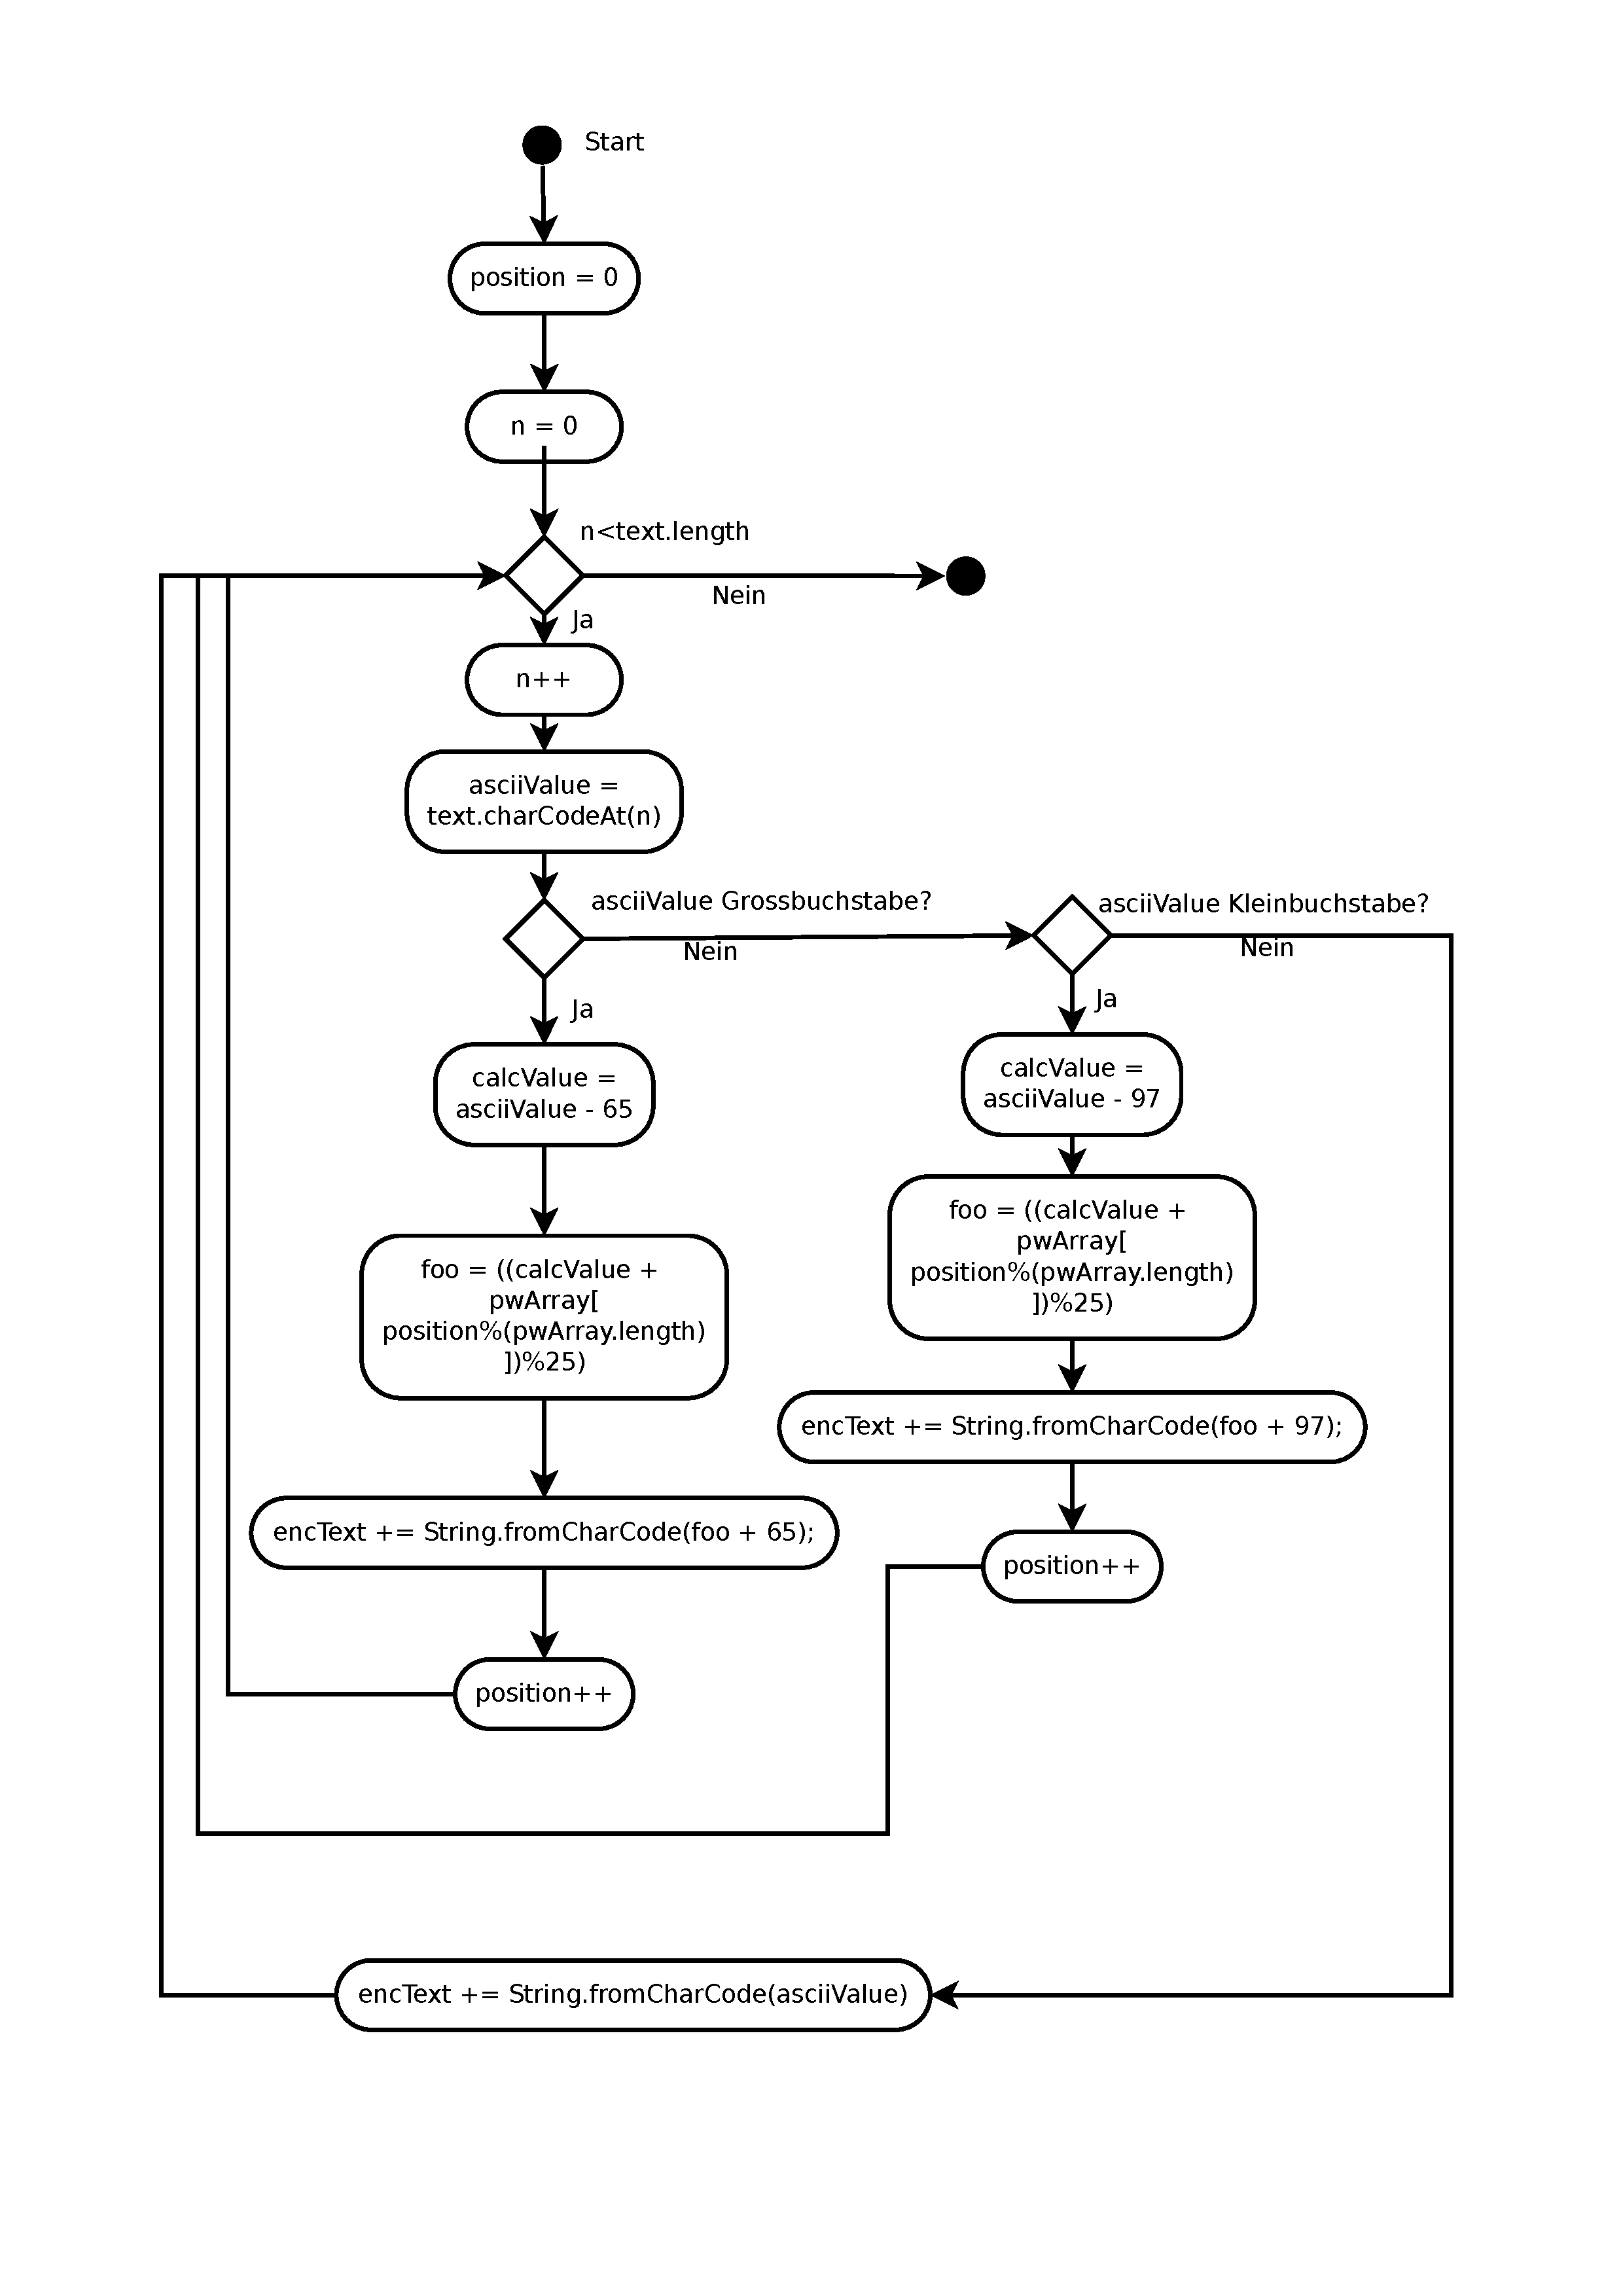
\includegraphics[width=\textwidth]{encrypt.pdf}
  \caption{UML Abbildung der Encrypt-Funktion}
  \label{fig:encrypt}
\end{figure}
\paragraph{decrypt}
Decrypt funktioniert sehr \"ahnlich wie die encrypt Funktion. Der einzige
signifikante Teil der sich ge\"andert hat, ist die Berechnung die so umgekehrt
wurde, dass der Text entschl\"usselt wird.
\begin{verbatimtab}
  var l=0;
  # indiziert, wie an welcher Stelle im Text wir uns befinden
  ...
  var calcValue = asciiValue-97
  # in ASCII, die kleinen Buchstaben beginnen bei 97. Die mathematische
  # Operation wird aber einfacher, wenn man Werte zwischen 0 und 25 verwendet
  # weshalb wir hier die 97 abziehen.
  var foo =
  (
    (
      26+calcValue-
      # die 26 die hier addiert werden, stellen sicher, dass wir durch die
      # folgende Substraktion nicht in einen negativen bereich fallen
      pwArray[l%(pwArray.length)]
      # Auslesen des Passworts-Zeichens der entsprechenden Stelle. Die
      # Modulo-Operation stellt sicher, dass, sobald das Ende des Arrays
      # erreicht ist, wieder von vorne begonnen wird.
    )
    %26
    # Der erreichte Wert muss zwischen 0 und 25 liegen. Deshalb wenden wir erneut
    # %eine Modulo-Operation an.
  )
  decText += String.fromCharCode(foo+97)
  # Zum Schluss f\"ugen wir die 97 wieder hinzu um einen brauchbaren ASCII Wert
  # zu erhalten. fromCharCode wandelt diesen Zahlenwert dann in eine Zahl um.
\end{verbatimtab}
\paragraph{preparePassword}
F\"ur die Funktionen encrypt und decrypt ist es einfacher, wenn das Passwort als
Array von Integern vorliegt als als Buchstaben. Deshalb wird es zuerst in die
Funktion \glqq preparePassword\grqq eingespielt, die es als Liste von
Zahlenwerten zur\"uckgibt. So muss in den ohnehin komplexen Formeln nicht auch
immer noch der Passwort-Wert umgerechnet werden. Ausserdem kann so
Rechenleistung gespart werden. Da das Passwort in der Regel k\"urzer ist als der
zu verschl\"usselte Text, wird jedes Zeichen des Passwortes mehrmals verwendet.
Dadurch, dass es zuvor einmal umgerchnet wird, muss nicht jedes Zeichen bei
jeder Verwendung wieder umgerechnet werden. Ausserdem stellt die Funktion
sicher, dass nur alphabetische Funktionen im verwendeten Passwort landen. Die
Funktion ist in Abbildung \ref{fig:preparePassword} \glqq
\nameref{fig:preparePassword}\grqq abgebildet.
\begin{figure}[h!]
  \centering
  \includegraphics[width=\textwidth]{preparePassword.pdf}
  \caption{UML Abbildung der preparePassword Funktion}
  \label{fig:preparePassword}
\end{figure}
\paragraph{visualSquare}
Diese Funktion erstellt zeichnet ein Vigen\`ere Square. Das sollte in etwa so
aussehen wie in Abbildung \ref{fig:square} \glqq \nameref{fig:square} \grqq
dargestellt.
\begin{figure}[h!]
  \centering
  
\includegraphics[width=0.6\textwidth]{square.png}
  \caption{Vigen\`ere Square}
  \label{fig:square}
\end{figure}

Dazu kommen noch einige weitere Funktionen die vorallem als Wrapper dienen um
die Verwendung zu vereinfachen oder bei der visuellen Darstellung behilflich
sind. Genaueres findet sich dann in der %TODO
\subsubsection{Oberfl\"achenentwurf}
\paragraph{Bedienelemente}
Die Applikation wird drei Eingabefelder darstellen. Das erste davon ist
lediglich einzeilig und f\"ur die Eingabe des Passwortes vorgesehen. Die beiden
anderen sind mehrzeilig und exakt gleich gross. Das eine davon enth\"alt den
unverschl\"usselten Text, das andere den verschl\"usselten. Zwischen den beiden
Feldern befinden sich zwei Kn\"opfe mit denen sich der Text verschl\"usseln,
respektive entschl\"usseln l\"asst. Grafik \ref{fig:interface} \glqq
\nameref{fig:interface} \grqq gibt einen Eindruck davon.
\begin{figure}[h!]
  \centering
  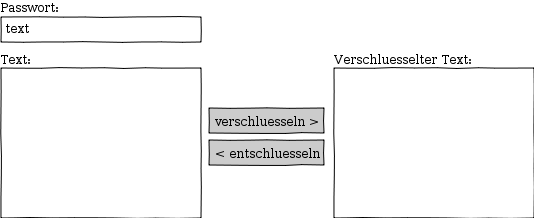
\includegraphics[width=0.8\textwidth]{interface.png}
  \caption{Entwurf der Programmoberfl\"ache}
  \label{fig:interface}
\end{figure}

\paragraph{Vigen\`ere Rechteck}
Das einzig andere wichtige Element ist das Vigen\`ere Rechteck. Mit dessen hilfe
wird der Algorithmus visualisiert. Dazu wird jeweils zum aktuellen Zeichen des
Passwortes die entsprechende Zeile und zum aktuellen Zeichen des Textes die
entsprechende Spalte markiert. Der Buchstabe im Treffpunkt der beiden
Markierungen wird ausgelesen. Grafik \ref{fig:select} \glqq \nameref{fig:select}
\grqq zeigt wie die Autoren sich das vorstellen.
\begin{figure}[h!]
  \centering
  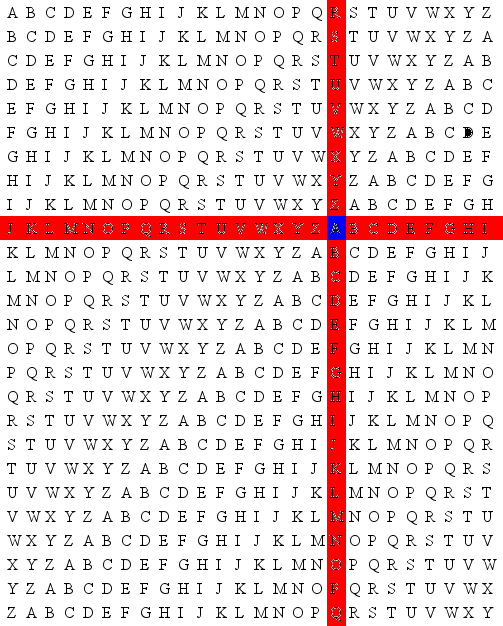
\includegraphics[width=0.8\textwidth]{select.png}
  \caption{Konzeptioneller Entwurf der Abbildung des Vigen\`ere Rechtecks}
  \label{fig:select}
\end{figure}


\subsubsection{Wikipedia-Eintrag}
\paragraph{Analyse \"ahnlicher Artikel}
Um einen geeigneten Aufbau f\"ur unseren Artikel zu bestimmen, haben wir
bestehende Wikipedia Eintr\"age zu \"ahnlichen Themen analysiert. Die
untersuchten Artikel sind:
\begin{itemize*}
  \item Caesar Verschl\"usselung
  \item Digital Signature Algorithm (DSA)
  \item RSA-Kryptosystem 
  \item Elliptic Curve Cryptography (ECC)
  \item Advanced Encryption Standard (AES) (auch rijndael)
  \item One-Time-Pad
\end{itemize*}
Hier sind die Ergbenisse dazu:

\subparagraph{Aufbau}
\begin{itemize*}
  \item viele der Artikel enthalten eine vereinfachende Grafik um den Ablauf der
  Verschl\"usselung grob zu umreissen
  \item Die untersuchten Artikel verf\"ugen \"uber einen Abschnitt, der den
  historischen Hintergrund des Algorithmus erl\"autert
  \item Allen gemeinsam ist auch, dass sie die Funktionsweise erkl\"aren
  \item Die Sicherheit und Analyse dieser wird als Kryptoanalyse bezeichnet und
  wird in der Regel in einem oder gar mehreren Kapitel behandelt
  \item Bei modernen und aktuellen Algorithmen werden meistens verschiedene
  Implementationen einzeln behandelt
\end{itemize*}
\subparagraph{Stil}
\begin{itemize*}
  \item Um die Funktionsweise sachlich korrekt zu beschreiben werden
  mathematische Hintergr\"unde beleuchtet und durch Formeln dargestellt
  \item Bei den simpleren Algorithmen kann ein einfaches Beispiel die
  Funktionsweise gut umschreiben
\end{itemize*}

Hier ist noch eine Analyse anhand einiger Zitate aus den Artikeln. Dies soll als
Hilfe bei der Formulierung unseres eigenen Textes dienen.

\begin{quote}
  \frqq Der öffentliche Schlüssel (public key) ist ein Zahlenpaar \((e,N)\) und
  der private Schlüssel (private key) ein Zahlenpaar \((d,N)\), wobei \(N\) bei
  beiden Schlüsseln gleich ist. Man nennt \(N\) den RSA-Modul, \(e\) den
  Verschlüsselungsexponenten und d den Entschlüsselungsexponenten.\flqq
  \footnote{\cite{wiki:Caesar-Verschluesselung}}
\end{quote}

An diesem Textbeispiel des RSA-Artikels ist gut ersichtlich, dass der Stil
sachlich und pr\"azise ist. Der Text ist vielleicht f\"ur den Laien nicht
unbedingt verst\"andlich - Der Artikel ist an Personen gerichtet, die bereits
\"uber Kenntnisse der Kryptographie verf\"ugen. Die Vigen\`ere-Chiffre ist
jedoch eher f\"ur Anf\"anger geeignet und wird auch oft als Beispiel dazu
gebraucht. Daher sollte unser Artikel verst\"andlicher und auch f\"ur Anf\"anger
gut verst\"andlich sein. Als Beispiel soll hier ein Ausschnitt aus dem Artikel
\"uber die C\"asar-Verschl\"usselung dienen, die auch oft als Einstieg in die
Kryptographie dient:

\begin{quote}
  \frqq Neben der Nutzung eines veränderten Alphabets, in dem etwa Ziffern und
  Sonderzeichen enthalten sind, gibt es zudem die Variante der umgekehrten oder
  revertierten Caesar-Verschlüsselung.\flqq
  \footnote{\cite{wiki:RSA-Kryptosystem}}
\end{quote}

\paragraph{Entwurf}
\begin{enumerate*}
  \item Einleitung
  \item Geschichte
  \item Einsatzgebiete
  \item Beschreibung der Funktionsweise
  \item Mathematische Funktionsweise
  \item Variationen
  \item Kryptoanalyse
\end{enumerate*}
%\section{Abstract}
%\section{Einleitung}
%Kryptografie ist ein wichtiges Teilgebiet nicht nur der Informatik, sondern auch
%der Mathematik. Es bietet ein praktisches und kommerzielles Anwendungsfeld f\"ur
%viele mathematische Grundlagen. Dabei ist korrekte und sichere Verschl\"usselung
%heute von sehr grosser Bedeutung. Ein Grossteil des Datenaustausches findet
%\"uber das Internet statt. Wer da noch mitliest, l\"asst sich nicht genau sagen.
%M\"ochte man Daten bei der \"Ubertragung deshalb geheim halten, so ist es
%wichtig, dass diese verschl\"usselt sind. Ausserdem ist eine gute
%Verschl\"usselung auch eine grosse Herausforderung. Die Rechenkraft von modernen
%Computern, besonders von Supercomputern schnellt seit Jahrzehnten in die H\"ohe.
%Die Paralellisierung der Rechenaufgabe und der Einsatz optimierter Hardware wie
%GPUs und FPGAs versch\"arfen die Situation weiter. Unsichere Verschl\"usselungen
%lassen sich so innert Sekunden knacken. Andererseits muss eine gute
%Verschl\"usselung auch auf rechenschwachenger\"aten wie Smartphones, Router oder
%gar Fernsehern funktionieren und das ohne, dass die Akkulaufzeit negativ
%beeinflusst wird.
%
%All das hat dazu gef\"uhrt, dass moderne Verschl\"usselungsalgorithmen wie ECC
%oder AES sehr komplexe mathematische Formeln sind. Die ganzen Zusammenh\"ange
%und den Aufbau solcher Verschl\"usselungen zu verstehen ist alles andere als
%trivial. Wer neu in das Feld der Kryptografie einsteigt, sollte sich zuerst mit
%einfacheren Konzepten auseinander setzen.
%
%Die Vigenere Verschl\"usselung ist aus heutiger Sicht zwar l\"angst veraltet und
%unsicher. Selbst vor dem Zeitalter von Computern war es, mit viel Aufwand,
%bereits m\"oglich, solche Verschl\"usselungen zu knacken. Trotzdem ist die
%Betrachtung sehr interessant. Die Schw\"ache des Algorithmus ist auf den ersten
%Blick nicht zu erkennen. Es l\"asst sich auch zeigen, wie viel einfacher
%Computer das Knacken schlechter Verschl\"usselungen machen.
%
%In dieser Arbeit stellen wir die Frage, wie Viegenere funktioniert und
%insbesondere, wie man dessen Funktionsweise einfach verstaendlich machen kann.
%Dazu soll eine visuelle Repr\"asentation der Funktion des Algorithmus erstellt
%werden. Wir wollen auch wisse, wieso denn der Algorithmus unsicher ist und wie
%man ihn knacken kann. Wie aufw\"andig ist das eigentlich? Da wir ohnehin eine
%visuelle Umsetzung des Algorithmus erstellen, die so funktioniert, wie ein
%Mensch sich das einfahc vorstellen kann, wollen wir die Performance dieses
%Vorgehens vergleichen, mit einer Implementation desselben Verfahrens mit
%mathematischen Formeln. Zuletzt stellt sich uns noch die Frage, wie einfach sich
%die Visualisation mit modernen Webtools umsetzen l\"asst.
%\section{Praxisarbeit}
%Zur Praxisarbeit z\"ahlt eine Webapplikation, die die Funktionsweise von
%Vigenere erl\"autert. Auch das 'knacken' der Verschl\"usselung geh\"ort zum
%Praxisteil und die dabei gemachten Erfahrungen werden hier erl\"autert.
%\section{Theorieteil}
%Der Theorieteil umfasst den Wikipediaartikel zu dem Thema, eine Erl\"auterung
%der Funktionsweise der Verschl\"usselung und eine Beschreibung der Schw\"achen
%des Algorithmus. Diese Schw\"achen werden mithilfe geeigneter
%Krypto-Analyse-Software getestet. Die dabei gewonnenen Erkenntnisse werden im
%Praxisteil erl\"autert.
%\newpage
%foo bar

\newpage

\listoftables
\listoffigures

\bibliography{arbeitsjournal.bib}{}
\bibliographystyle{plain}
\end{document}
